\documentclass[a4paper,10pt]{article}
\usepackage[top=2cm, bottom=2cm, left=2cm, right=2cm]{geometry}
\usepackage{amsmath}
%\usepackage{sydewkrpt}
\usepackage[pdftex]{graphicx}
\usepackage[latin1]{inputenc}
\usepackage{tikz}
\usetikzlibrary{shapes,arrows}
\usepackage{caption}
\usepackage{multirow}
\usepackage{graphicx}
\usepackage[space]{grffile}
\usepackage{float}
\usepackage{multicol}
\usepackage{helvet}
\usepackage{sectsty}

\restylefloat{table}
\restylefloat{figure}

\renewcommand{\thesection}{\arabic{section}}
\renewcommand{\labelitemi}{$\bullet$}
\everymath=\expandafter{\the\everymath\displaystyle}
\newcommand{\Lagr}{\mathcal{L}}
\renewcommand{\familydefault}{\sfdefault}
\sectionfont{\centering\bf\sc}

\begin{document}
\pagenumbering{gobble}

\begin{center}
	\textbf{ \textsc{ \Large Relay: Adaptive Traffic Control Framework}}\\
	[6pt]
	\textbf{ \large Alexander Huras, D. Scott Neil, Myles Tan, Riley Donelson}\\
	\textbf{\large Dr. Bruce Hellinga}\\
	\large Department of Systems Design Engineering
\end{center}

\begin{abstract}
Relay is a research and design project focused in the domains of Adaptive Traffic Control and Data Visualization.
In recent years, multiple cities including Montreal and LA have begun to implement adaptive systems, but adoption is not widespread.
This shows a great deal of potential in maturing this technology further.
The Relay Framework is a distributed traffic controller, leveraging peer-to-peer, and agent-based modelling technologies.
Intersections communicate with one another, constantly gathering and sharing information, and propagating local insight through the network.
When combined with powerful predictive algorithms, Relay is able to quickly adapt to changing traffic conditions.
The Relay Interface democratizes traffic data, enabling a common understanding of traffic patterns, giving both public offices and citizens the ability to make informed decisions.
By providing insightful information on intersection statistics and traffic patterns, the Relay Interface offers a window into cities that has never been seen before.
\end{abstract}

\begin{multicols}{2}
\setlength{\parskip}{6pt}

\section{Background Information}
Motorists and pedestrians alike can relate to the frustration of being stopped unnecessarily at a red light, with no other cars in sight.
Large metropolitan areas are acknowledging the need for advanced traffic systems as size and density of urban areas increases.
For example, Los Angeles has developed a solution to handle the massive volume placed on their transportation networks, at an estimated cost of \$400 million to date \cite{la-atcs-article}.
There is strong need for ATCS technology in the world today, and a large opportunity for state-of-the-art ATC systems.

The intelligence of a traffic light varies from a static, fixed timer, to an intelligent node which considers existing traffic conditions, performance of adjacent nodes, and the like.
Multiple industry-accepted ATC systems exist, such as LA ATCS, SCOOT, Trafficware, and Spectrum by Miovision.
However, high implementation costs are often a deterrent from implementing such systems.
Additionally, research efforts in academia are being made towards novel architectures such as agent-based distributed systems, which implement advanced machine learning and neural network concepts\cite{1688100, 5073360, uot-article}.
There still exists a large gap between academia and industry, showing potential for the incorporation of cutting edge solutions into municipal infrastructure.

\section{\textsc{Problem \& Requirements}}
%maybe change this to just a problem statement to shorten it

Access to data from ATCS systems is largely kept for internal analysis by government organizations, suffocating further technological development by industrial and academic organizations.
Additionally, no existing systems offer public access to the systems data, in any form.

The solution must meet the needs of transportation authorities, who will be responsible for overseeing performance and maintenance, and are ultimately responsible for the system.
The solution must also meet the needs of the public, providing transparent access to its operation and allowing consumers to take full advantage of the information.
Additionally, the system must implement acyclic, adaptive control patterns, utilizing distributed computation and peer-to-peer modeling technologies.
The advantages of the system should be apparent and noticeable by both stakeholders, and finally, the system must be reliable and robust, due to the severe safety and efficiency consequences of failure and poor performance. 
The Relay system will be a proof of concept for \emph{democratic}, distributed intelligent traffic control systems.

\section{\textsc{Relay Interface}}

% if we have space, this figure can be included
\begin{figure}[H]
  \begin{centering}
    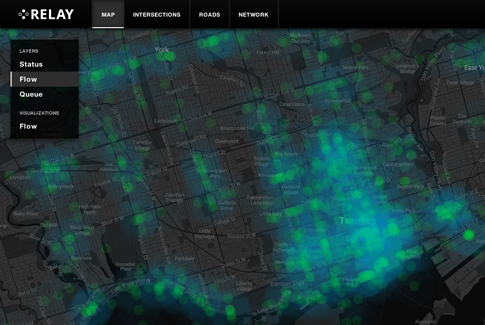
\includegraphics[scale=0.35]{figures/flow-2.png}
    \caption{Screenshot from the Relay Interface.}
    \label{fig:interface}
  \end{centering}
\end{figure}

%brief overview of what is provided
The Relay Interface has helped redefine the value of Adaptive Traffic Control System Interfaces. For Traffic Engineers, the application enables the shift of responsibility and value from signal timing and tweaking, to network monitoring and informed planning. Relay Interface exposes rich information which was previously either impossible or extremely expensive to collect, greatly reducing costs associated with maintaining efficiency of the network. This information allows traffic engineers to know exactly what's going on in the network at any moment. Through the use of geospatial data visualizations, the application is able to reveal high-level traffic patterns, providing invaluable insight into the workings of a city's transportation network. Access to this kind of information has the potential to change the way public infrastructure decisions are made. This project should serve as a guide for the development of Adaptive Traffic Control System Interfaces in the future.



\section{\textsc{Relay Framework}}

In Relay, each intersection is governed/controlled by its own independent, autonomous controller or \emph{Agent}.
At its heart, each Agent in a Relay network is a dynamic graph automata---responsible for interpreting and propagating (transformed) sensor measurements to its neighbours.
In addition to informing its peers of local environmental measurements (such as vehicles incident at their controlled intersection), Relay Agents generate and propagate \emph{predictions} or \emph{expectations} of traffic flow through their region, modulating and transforming the predictions received from peers in light of their expected signal timing schedule.
The Agents continuously (via reinforcement learning) update their internal models to match the current environmental dynamics such that the prediction error is minimized.

Simultaneously each agent continually adjusts and optimizes its signal timing schedule (i.e. alternating ``Red'' and ``Green'' states for an arbitrary direction) based on the transformed predictions of its peers, congruent to a (relatively) straightforward Mixed-Integer Nonlinear Dynamic Programming routine, that takes into account dynamical queue simulations and probabalistic uncertainty associated with the predictions.

Ultimately, as a Framework (the abstracted Agent parameterization), Relay offers a platform for implementing abstract traffic controllers that leverage state-of-the art optimization, and machine learning algorithms.


\section{\textsc{Impacts}}
Adaptive Traffic Control Systems have many positive social and environmental implications as a byproduct of improving traffic flow through a city.
A few of these are decreased gas consumption, reduced travel time, and reduced congestion.
It is important to note that these are not direct goals of the implementation, but rather beneficial external consequences of effective traffic control, that naturally extend from effectively adapting signal timings.
The proposed solution thus focuses on local intersection performance, which in turn contributes to the improvement of aforementioned social and environmental benefits.

\section{\textsc{Conclusions}}
The push for democratized traffic data is a major goal for this project, and Relay Interface serves as a first major attempt to present infrastructure-quality traffic information to the public. 
Relay Interface allows the public to examine and understand the workings of their public infrastructure, encouraging a more informed and engaged population.

Additionally, with the formalization of the Relay Agent, we have outlined a generic and flexible platform for traffic engineers and researchers to experiment with the implementation of distributed traffic control systems that operate on probabilistic expectations, sparse-distributed computation, and \emph{soft}-synchronisation.
The Relay pattern additionally removes the necessity to have detailed information about the implementation environment, with enough data, the system will \emph{learn} its environmental parameters, and provide full transparency to the engineer.
With the prototype implementation we showed it was possible to implement the Relay pattern, with entirely open-source tools.
The creation of the Relay Network has helped further the understanding and capabilities of not only adaptive traffic control, but traffic control in general, with systems like Relay, the cognitive burden typically associated with large scale traffic engineering has been almost entirely removed---foreshadowing a paradigm shift (or possibly an identity crisis) in traffic engineering.

\section{\textsc{References}}
\bibliographystyle{IEEEtran}

\bibliography{bib}

\end{multicols}
\end{document}